\label{sec:gnn_robust_and_faulty_modes}

% We identify GNN failure modes in overfitting to noisy labels: (a) model is over-parameterized for task complexity, (b) input graphs are of low-order with a small number of nodes (c) low number of class labels in a dataset.
% We identify that GNNs are robust. However, when the task is too simple or sparse GNNs tend to overfit and memorize noisy labels, specifically when a model is over-parameterizated, or dataset contains low-order graphs, or few class labels.

% Our investigation relies on prior observations that underparameterized models are more robust to label noise compared to overparameterized models \cite{memorizenoise}. 
% In our experiments, we took into account GNN smoothness inductive bias, 
%\cite{} \textcolor{red}{TO BE ADDED SMOOTHNESS BIAS INTO RELATED WORK AND HERE}
% which contributes to the robustness of GNN. Still, our investigation discovered the following failure modes:
%These studies suggest that a model during training is more likely to focus on generalized patterns rather than fitting on outlying the noise, with GNN's additional tendency to smooth over data. 
% We observe that aspects of task and model complexity affect GNN's robustness to noise. Specifically, our experiments show that with a fixed model, as task complexity decreases, the model increasingly overfits on noise,  suggesting that the more over-parameterized a model is relative to a simple task, the more it tends to memorize noise rather than generalizing effectively.

% \begin{figure}[htbp]
%     \centering   
%     %\includegraphics[scale = 0.3]{Neurips/Screenshots/synthetic_data/PPaClassChange_20N_30data.png}
%     %
\includegraphics[page=1,width=.5\textwidth]{Neurips/figures/fig3}
%     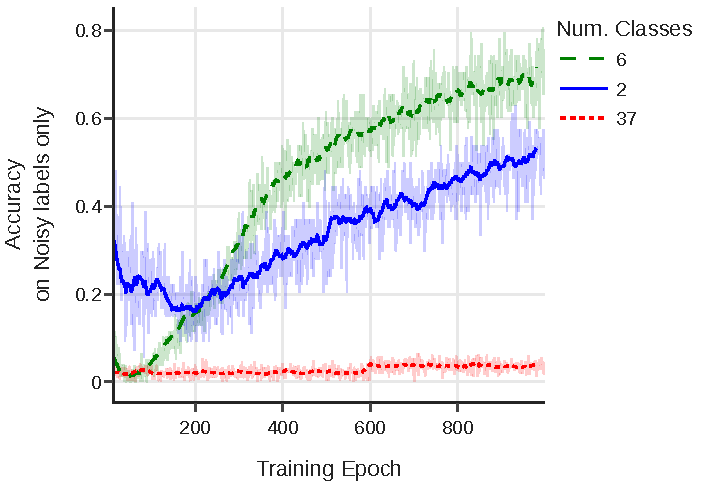
\includegraphics[page=1,width=.5\textwidth]{AISTATS/figures/fig3}
%     \caption{Performance only on noisy labels depending on the number of classes sampled from the PPA dataset. The binary 2-call case fits less on noise than the 6-class, since the binary case has only symmetric, more contrasting noise.}
%     \label{fig:ppa_changing_number_of_classes}
% \end{figure}
% \begin{figure}[htbp]
%     \centering   
%     %
\includegraphics[page=1,width=.5\textwidth]{Neurips/figures/fig2.pdf}
%     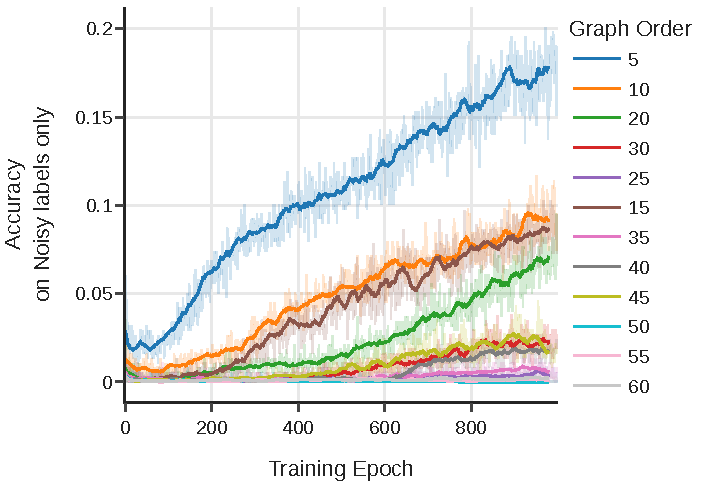
\includegraphics[page=1,width=.5\textwidth]{AISTATS/figures/fig2}
%     \caption{Performance only on noisy labels depending on graph order (number of nodes per graph). As training progresses, on low-order graph datasets, GNNs quickly overfit on noise (higher noise labels accuracy).}
%     \label{fig:synthetic_data}
% \end{figure}

% \begin{figure}[htbp]
%     \centering   
%     %\includegraphics[scale = 0.3]{Neurips/Screenshots/synthetic_data/PPa_SamplesNumber_40.png}
%     %
\includegraphics[page=1,width=.5\textwidth]{Neurips/figures/fig4}
%     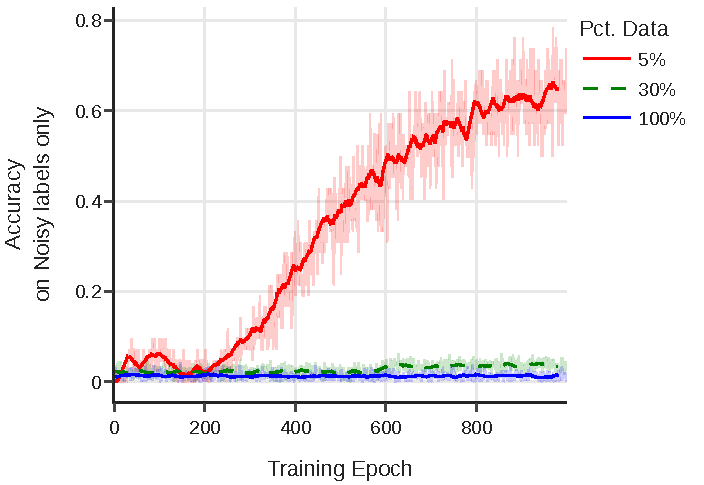
\includegraphics[page=1,width=.5\textwidth]{AISTATS/figures/fig4}
%     \caption{Performance only on noisy labels depending on the size of sampled PPA. Smaller datasets are more prone to memorization and fitting on noise.}
%     \label{fig:ppa_changing_number_of_smaples_of_class}
% \end{figure}



\begin{figure*}
    

    \centering
    % \setcounter{figure}{4} 
    
    \subfigure[ ]
    {
        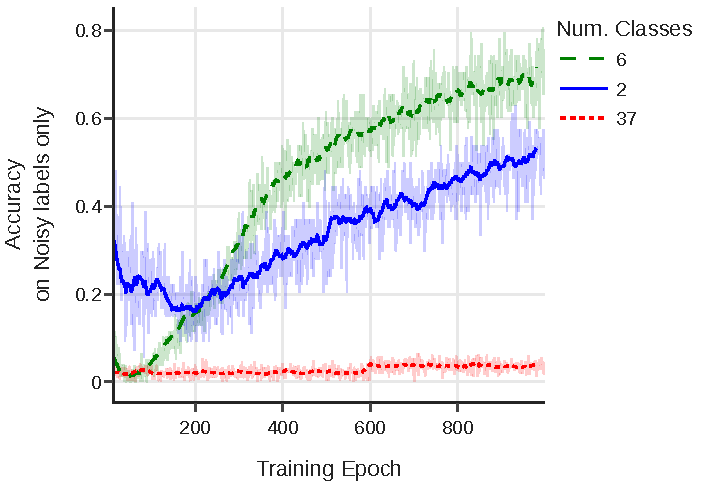
\includegraphics[width=0.45\textwidth]{AISTATS/figures/fig3}
        \label{fig:ppa_changing_number_of_classes}
    }
    \subfigure[]
    {
        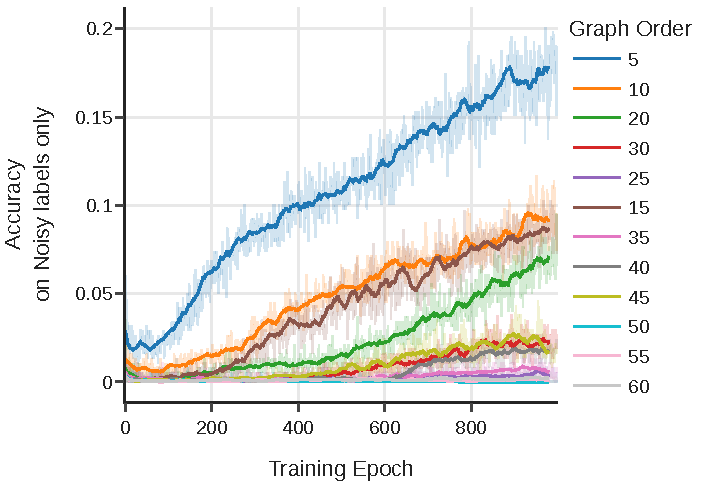
\includegraphics[width=0.45\textwidth]{AISTATS/figures/fig2}
         \label{fig:synthetic_data}
    }
    % Main figure caption (will still be figure 5)
    \caption{
    Training accuracy on noisy labels only. Effect of dataset properties: (a) Fewer classes in PPA lead to faster overfitting on noise. (b) Lower graph order leads to faster overfitting on noise..
    % Training accuracy on only noisy labels. 
    % Effect of dataset properties on noisy label learning
    % % \ref{fig:ppa_changing_number_of_classes} 
    % (a) Varying the number training classes in PPA dataset, lesser classes lead to faster overfitting on noise % \ref{fig:synthetic_data}:%
    % (b) Varying the graph order of training graphs, lower order lead to faster overfitting on noise
    }
    \label{fig:various_figures}
\end{figure*}

\begin{figure}[htbp]
    \centering
 \subfigure[]
    {
        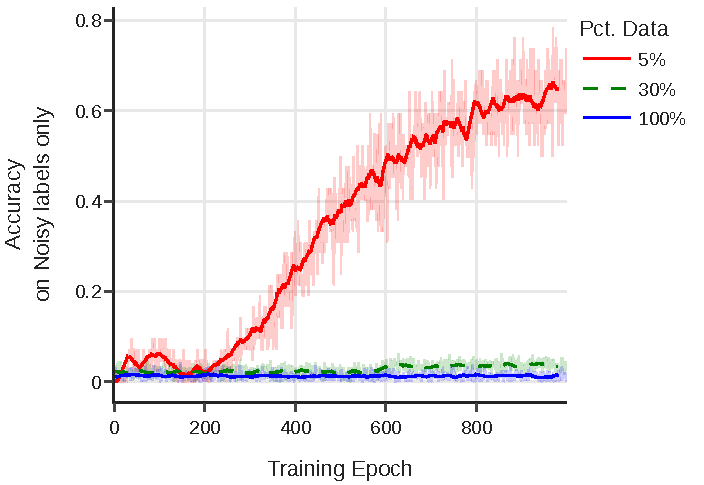
\includegraphics[width=0.45\textwidth]{AISTATS/figures/fig4}
        \label{fig:ppa_changing_number_of_smaples_of_class}
    }
        \subfigure[]
    {
        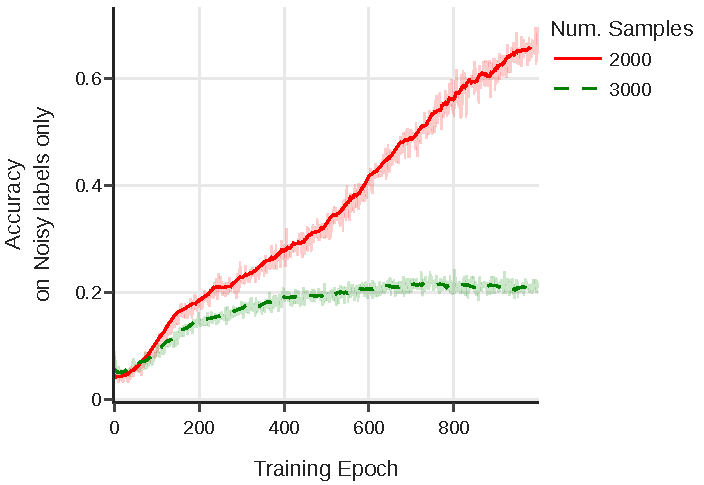
\includegraphics[width=0.45\textwidth]{AISTATS/figures/fig5}
        \label{fig:varying_samples_synthetic}
    }
    % Main figure caption (will still be figure 5)
    \caption{Training accuracy on noisy labels only. Effect of dataset size: (a) Smaller fractions of the PPA dataset lead to stronger noise memorization. (b) Smaller synthetic datasets are also more prone to memorizing noise.}
\end{figure}

% \begin{figure}[ht]
%     \centering
%     %\includegraphics[scale = 0.3]{Neurips/Screenshots/synthetic_data/sampleNumber.png}
%     %
\includegraphics[page=1,width=.5\textwidth]{Neurips/figures/fig5}
%     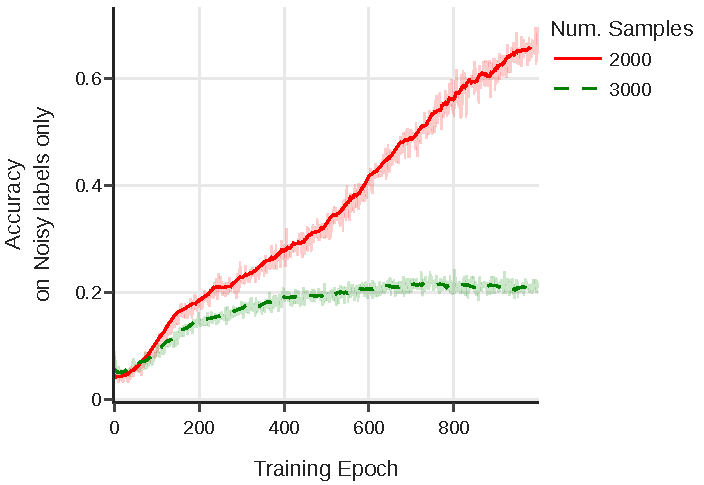
\includegraphics[page=1,width=.5\textwidth]{AISTATS/figures/fig5}
%     \caption{Performance only on noisy labels depending on the size of a synthetic dataset.}
%     \label{fig:varying_samples_synthetic}
% \end{figure}
% \begin{figure}[htbp]
%     \centering   
%     %
\includegraphics[page=1,width=.5\textwidth]{Neurips/figures/fig2.pdf}
%     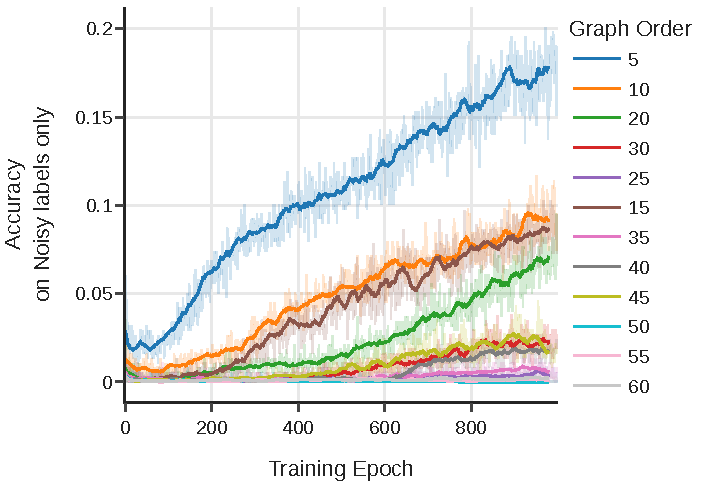
\includegraphics[page=1,width=.5\textwidth]{AISTATS/figures/fig2}
%     \caption{Performance only on noisy labels depending on graph order (number of nodes per graph). As training progresses, on low-order graph datasets, GNNs quickly overfit on noise (higher noise labels accuracy).}
%     \label{fig:synthetic_data}
% \end{figure}
% \begin{figure}[t]
%     \centering   
%     %\includegraphics[scale = 0.3]{Neurips/Screenshots/synthetic_data/PPa_SamplesNumber_40.png}
%     %
\includegraphics[page=1,width=.5\textwidth]{Neurips/figures/fig4}
%     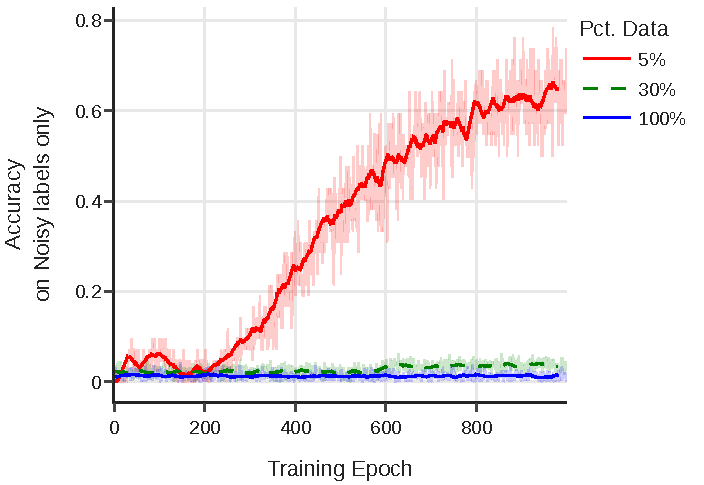
\includegraphics[page=1,width=.5\textwidth]{AISTATS/figures/fig4}
%     \caption{Performance only on noisy labels depending on the size of sampled PPA. Smaller datasets are more prone to memorization and fitting on noise.}
%     \label{fig:ppa_changing_number_of_smaples_of_class}
% \end{figure}
% Even with their smoothing bias, GNNs can fail under certain conditions of label noise. We systematically study when a GNN overfits noisy labels. Our findings reveal three main failure modes:
% \textbf{1. GNNs are not robust on simpler tasks (proxy to over-parameterized model overfitting).}
% Our investigation relies on prior observations that underparameterized models are more robust to label noise compared to overparameterized models \cite{memorizenoise}. 
% To study how model and task complexity relate, we choose a strategy of keeping the model fixed and measuring its performance for different scales of related tasks. In this experiment, we use the PPA \cite{PPA} dataset with a sub-sampled number of classes: 2, 6, and full 37 classes. As we reduce the number of classes, not only does the dataset size decrease, but the model also learns fewer classes to separate. We reduce the task complexity by decreasing number of its classes, resulting in a simpler PPA dataset while preserving all its other properties. The results in Fig. \ref{fig:ppa_changing_number_of_classes} show GNN training accuracy computed only for the noisy (mislabeled) graph labels per each training epoch. These curves in this and the following experiment, show how overfitting on noise emerges during the training process. In this case, for the most difficult task (37 classes) the model is underparametraised, hence does not memorize individual samples and does not fit on noise. Conversely, for the simpler task (6- and 2-class datasets) the model fits on noisy samples. Notice, the 2-class binary classification case is less susceptible to noise fitting than the 6-class dataset. The prime cause is that in the binary dataset we have only symmetric noise, which allows the model to better differentiate the contrasting mislabeled samples. 

% Notice that we use only 30\% of the PPA dataset to induce higher noise susceptibility (see below dataset size impact). As for the \emph{noise injection} method, we switch 20\% of labels from the original to a random alternative label, chosen uniformly from the other classes. The \emph{model} used is a 5-layered Graph Isomorphism Network (GIN) \cite{WL1} of 300 hidden units. 
% % \end{enumerate}

% \textbf{2. GNNs are not robust on low-order graphs.}
% Results in Fig. \ref{fig:synthetic_data} show that GNN becomes susceptible to noise as graph order decreases (i.e. lower number of nodes per sample graph). 


% To create the experiment setup, we generated synthetic datasets with an average \emph{Graph Oder} ranging from 5 to 60 nodes, drawing specific node counts from a Poisson distribution with $\lambda =$ \emph{Graph Oder}. Overall, each generated \emph{Dataset} contains 6 graph classes with 1400 sample graphs each. The graphs have average degree fixed at 2, the edges are created by selecting uniformly at random node pairs.
% %, and the number of edges scales with nodes.
% \emph{Node Feature} is sampled from Gaussian with $\mu = f(\textrm{graph label})$ and $\sigma = 1.5$. The noise rate is constant across the datasets: for each dataset we flipped 35\% of labels choosing uniformly from the other classes.


% \textbf{3. GNNs are not robust on small training sets.}
% %\textbf{THE MORE SAMPLES = the harder to memorise them}
% Finally, we isolate the impact of the dataset size on the noise robustness. We evaluate both datasets employed before. For the PPA dataset, we use all classes, and sub-sampled labels in each class to vary the dataset size. The results with the introduced {20\% noise} are shown in Fig. \ref{fig:ppa_changing_number_of_smaples_of_class}. 
% We also test the previously described synthetic dataset of 6 classes, with graph order 7. The results with 35\% noise are shown in Fig. \ref{fig:varying_samples_synthetic} in the Appendix \ref{appendix:additional_figures}, where you can find additional figures further supporting the main observations.

% Across the datasets, the experiments confirm that as the number of samples decreases, the model tends to overfit the noisy labels more rapidly.
We study when and why a GNN applied to graph classification overfits noisy labels.
Interestingly, GNNs exhibit a degree of inherent robustness. For instance, injecting noise into the full PPA  dataset ~\citet{PPA}, or large portions of it, does not significantly degrade model performance (see Fig.  \ref{fig:ppa_changing_number_of_classes}, \ref{fig:ppa_changing_number_of_smaples_of_class}, \ref{fig:noisy_pure_40_1}). 
We hypothesize that the observed robustness on PPA stems from the fact that the models may be under parameterized for the inherent difficulty of the PPA benchmark, on which state of the art methods struggle to achieve perfect accuracy\footnote{\url{https://paperswithcode.com/sota/graph-property-prediction-on-ogbg-ppa}}. This finding aligns with general findings that under parameterized models are often more robust to noise \citep{memorizenoise}.
Despite this, we show that GNNs nevertheless fail under certain conditions of label noise. To examine this, we fix the model architecture and manipulate task complexity by (i) varying the number of classes as a proxy for over-parameterization, (ii) varying the average number of nodes in synthetic datasets, and (iii) varying the share of training data used. We study the average training accuracy on noisy labels as a direct measure of how much the model fits noise. Higher accuracy on noisy samples indicates the model is memorizing them, while lower accuracy suggests that the model is not fitting the noise.

\textbf{GNN Robustness varying number of classes }
We use 30\% of the PPA dataset and inject 20\% symmetric noise into this subset by randomly replacing labels with uniformly sampled incorrect classes. The model here and below, if not said otherwise, is a 5-layer Graph Isomorphism Network (GIN)~\citet{WL1} with 300 hidden units.
Specifically, we create a sub-sampled PPA dataset with 2, 6, and the full 37 classes. Intuitively, reducing the number of classes simplifies the classification task and reduces the effective dataset size, making the fixed model increasingly overparameterized relative to the task.
Fig. ~\ref{fig:ppa_changing_number_of_classes} shows the training accuracy on noisy samples across epochs. For the full 37-class task, the GNN does not memorize noise and remains relatively robust. However, when the number of classes is reduced to 6 and further to 2, the model increasingly fits the noisy labels. Interestingly, the 2-class case exhibits slightly more robustness than the 6-class case due to the symmetric nature of the injected noise, since random flipping between two classes produces highly contrasting noisy samples.

\textbf{GNNs are not robust on low-order graphs.}  
We generated synthetic datasets (see procedure in Appendix, Section \ref{appendix:details_synthetic_dataset_varying_nodes}) to study the effect of graph order (number of nodes). As shown in Fig. ~\ref{fig:synthetic_data}, GNNs become increasingly sensitive to noise as the graph order decreases. Small graphs lack sufficient internal structure and aggregation capacity, making them vulnerable to treating noisy labels as signals. Conversely, larger graphs provide more nodes over which the model can average, diluting the influence of noisy samples.


\textbf{GNNs are not robust on small training sets.}  
The size of a training set affects the robustness to noisy labels. For the PPA dataset, we keep all 37 classes, but subsample the number of training graphs per class. As shown in Fig. ~\ref{fig:ppa_changing_number_of_smaples_of_class}, reducing the number of training samples increases the likelihood of overfitting noise. A similar trend is observed for the synthetic datasets (with graph order 7 and 6 classes) under 35\% label noise, as shown in Fig.~\ref {fig:varying_samples_synthetic}. In both cases, models trained on smaller datasets have a higher tendency to memorize noisy samples due to insufficient clean data to learn generalizable patterns.







%\textcolor{red}{REMOVE: Once we establish that for a model to effectively learn the graph classification task, the Dirichlet energy of the classes, as defined in equation \ref{eq: avg_dirichlet}, must decrease, while for models fitting noise, it tends to increase. To delve deeper into the correlation between fitting noisy samples and enhancing model smoothness, we delve into the significance of weight eigenvectors, elaborating on the importance of increased smoothness. Further discussion on this topic is provided in the subsequent section.}

